\documentclass[12pt, letterpaper]{report}
\usepackage{enumitem}
\usepackage[a4paper, margin=0.7in, top=20mm, bottom=20mm]{geometry}
\usepackage{mathspec}
\usepackage[UTF8]{ctex}
\usepackage[colorlinks=true, linkcolor=black, urlcolor=blue]{hyperref}
\usepackage{listings}
\usepackage{xcolor}
\usepackage{graphicx}
\usepackage{xparse}
\usepackage{tcolorbox}
\usepackage{mdframed}

\graphicspath{ {./pics/} }

% ---- Code Section Style ----
\colorlet{mygray}{black!30}
\colorlet{mygreen}{green!60!blue}
\colorlet{mymauve}{red!60!blue}

\tcbuselibrary{breakable}
\NewDocumentCommand{\exercise}{ m +m }{
    {
        \edef\originalParIndent{\the\parindent}
        \begin{tcolorbox}[breakable,arc=0mm,boxrule=0.8pt]
            \setlength{\parindent}{\originalParIndent}
            \noindent
            \textbf{\large Exercise #1}
            \indent
            #2
        \end{tcolorbox}
    }
}

\tcbuselibrary{breakable}
\NewDocumentCommand{\question}{ m +m }{
    {
        \edef\originalParIndent{\the\parindent}
        \begin{tcolorbox}[breakable,arc=0mm,boxrule=0.8pt]
            \setlength{\parindent}{\originalParIndent}
            \noindent
            \textbf{\large Question}
            \indent
            #2
        \end{tcolorbox}
    }
}

\tcbuselibrary{breakable}
\NewDocumentCommand{\challenge}{ m +m }{
    {
        \edef\originalParIndent{\the\parindent}
        \begin{tcolorbox}[breakable,arc=0mm,boxrule=0.8pt]
            \setlength{\parindent}{\originalParIndent}
            \noindent
            \textbf{\large Challenge!}
            \indent
            #2
        \end{tcolorbox}
    }
}

\lstdefinelanguage
   [x64]{Assembler}     % add a "x64" dialect of Assembler
   [x86masm]{Assembler} % based on the "x86masm" dialect
   % with these extra keywords:
   {morekeywords={CDQE,CQO,CMPSQ,CMPXCHG16B,JRCXZ,LODSQ,MOVSXD, %
                  POPFQ,PUSHFQ,SCASQ,STOSQ,IRETQ,RDTSCP,SWAPGS, %
                  rax,rdx,rcx,rbx,rsi,rdi,rsp,rbp, %
                  r8,r8d,r8w,r8b,r9,r9d,r9w,r9b, %
                  r10,r10d,r10w,r10b,r11,r11d,r11w,r11b, %
                  r12,r12d,r12w,r12b,r13,r13d,r13w,r13b, %
                  r14,r14d,r14w,r14b,r15,r15d,r15w,r15b}} % etc.


\lstset{
  backgroundcolor=\color{gray!10},  
  basicstyle=\ttfamily,
  columns=fullflexible,
  breakatwhitespace=false,      
  breaklines=true,                
  captionpos=b,                    
  commentstyle=\color{mygreen}, 
  extendedchars=true,              
  frame=single,                   
  keepspaces=true,             
  keywordstyle=\color{blue},                    
  numbers=none,                
  numbersep=5pt,                   
  numberstyle=\tiny\color{blue}, 
  rulecolor=\color{mygray},        
  showspaces=false,               
  showtabs=false,                 
  stepnumber=5,                  
  stringstyle=\color{mymauve},    
  tabsize=3,                      
  title=\lstname                
}

\lstdefinestyle{CStyle}{  
    % commentstyle=\color{mGreen},
    % keywordstyle=\color{magenta},
    % numberstyle=\tiny\color{mGray},
    % stringstyle=\color{mPurple},
    basicstyle=\footnotesize,
    breakatwhitespace=false,                              
    showstringspaces=false,
    language=C
}

\lstdefinestyle{AssemblyStyle}{  
    basicstyle=\footnotesize,
    breakatwhitespace=false,                              
    showstringspaces=false,
    language=[x64] Assembler
}


\lstdefinestyle{MakeFileStyle}{  
    basicstyle=\footnotesize,
    breakatwhitespace=false,                              
    showstringspaces=false,
    language=[gnu] make
}


\setitemize[1]{itemsep=0pt,partopsep=0pt,parsep=\parskip,topsep=5pt}

% ----------------------------


\setcounter{chapter}{0}
\setlength{\parindent}{2em}
\setmainfont{Times New Roman}
\setcounter{tocdepth}{1}
\setcounter{secnumdepth}{1}

\title{MIT6.828 Lab4: Preemptive Multitasking}
\author{Zhuofan Zhang}
\date{April 2022}



\begin{document}

\maketitle
% ---- Contents ----
\pagenumbering{roman}
\renewcommand\contentsname{\Huge Contents}
\tableofcontents{}
% ------------------

\newpage
\pagenumbering{arabic}

% ---- part A ----
\chapter[\Large Multiprocessor Support and Cooperative Multitasking]{Multiprocessor Support and Cooperative Multitasking}
\section[\large Multiprocessor Support]{Multiprocessor Support}
本次Lab的内容是对JOS进行补充以提供多处理器支持,并实现任务调度功能。\par

JOS实现的多核支持属于\textsl{对称多核支持(Symmertric Multiprocessing, SMP)},即所有处理器
对资源(内存、IO总线等)的访问是平等的。SMP的概念是在系统初始化完成后建立的,
在Boot阶段,仍然需要选择一个CPU作为\textsl{启动处理器(Bootstrap Processor, BSP)},用来初始化
资源并启动OS,最后启动其他的CPU(称为\textsl{应用处理器(Application Processor, AP)})。
对BSP的选择是由BIOS完成的,在当前实验阶段,我们相当于完成了BSP的启动内容。\par 

在SMP体系中,每个CPU都拥有一个称为LAPIC(local Advanced-Programmable Interrupt Controller)的可编程中断单元,用于在系统中
传递中断信息,并提供CPU的唯一识别信息。因此,与多个CPU的通讯依赖于LAPIC单元。 \par

在本次实验中我们使用了 LAPIC 的如下功能:
\begin{itemize}
    \item[·]
    代码可以利用APIC-id确认自己运行于哪一个cpu上(见 cpunum() 的实现)
    \item[·]
    利用BSP来启动其他的AP(见 lapic\_startap() 的实现)
    \item[·]
    使用 LAPIC 中的时钟中断来实现抢断式调度(PartC,apic\_init())
\end{itemize}

CPU对LAPIC单元的访问使用的是一段映射到PAS特定位置的区域:memory-mapped I/O (MMIO)。MMIO是一段
硬连接到部分IO设备寄存器的物理地址区域,常用于访问设备的寄存器。JOS的VAS在MMIOBASE处
留有4MB的空间用于映射这段物理地址区域。\par
\newpage
\exercise{1}{
        \par 
        {
            Implement mmio\_map\_region in kern/pmap.c. 
            To see how this is used, look at the beginning of lapic\_init in kern/lapic.c. 
            You'll have to do the next exercise, too, 
            before the tests for mmio\_map\_region will run.
        } \par
}
\quad \par
这一个Exercise要求我们实现mmio\_map\_region()。我们查看该函数的注释可知,它就是用来
实现上文提到的MMIO在VAS中映射的函数。JOS的VAS中预留了 [MMIOBASE, MMIOLIM) 可供使用。
根据提示使用 boot\_map\_region() 并补上禁用缓存的PWT-flag,实现函数如下:\par 
\lstset{style=CStyle}
\setmainfont{Consolas}
\begin{lstlisting}
void *
mmio_map_region(physaddr_t pa, size_t size)
{
    static uintptr_t base = MMIOBASE;

    size = ROUNDUP(size, PGSIZE);
    if(base + size > MMIOLIM)
        panic("mmio_map_region: MMIOLIM overflow.\n");
    boot_map_region(kern_pgdir, base, size, pa, PTE_W | PTE_PCD | PTE_PWT);
    base += size;
    return (void *)(base - size);
    
}
\end{lstlisting}
\setmainfont{Times New Roman}

\section[\large Application Processor Bootstrap]{Application Processor Bootstrap}
在启动APs前,先启动的BSP必须能够获取APs的信息,如CPU数量、APIC IDs等。
这些信息被保留在BIOS中的 MP config table 中,kern/mpconfig.c/mp\_init() 
将其读出。\par 
kern/init.c/boot\_aps() 是整个流程的核心函数,它将AP的入口程序加载到内存,
并发送启动信号。AP的入口程序被加载到任意可用的低位640k地址(JOS将其加载到MPENTRY\_PADDR),
它与BSP的入口程序有一定的区别。 \par 
boot\_aps() 函数通过给每个AP的LAPIC发送STARTUP信号的方式唤醒它们,同时设置它们的entry位置,
即为AP准备的入口程序(位于MPENTRY\_PADDR),执行完入口程序后AP将运行mp\_main();与此同时,
BSP唤醒每一个AP时等待它的CPU状态被设置为CPU\_STARTED——即该AP成功启动后,再开始唤醒下一个AP。\par 

\newpage
\exercise{2}{
        \par 
        {
            Read boot\_aps() and mp\_main() in kern/init.c, 
            and the assembly code in kern/mpentry.S. 
            Make sure you understand the control flow transfer 
            during the bootstrap of APs. 
            Then modify your implementation of page\_init() 
            in kern/pmap.c to avoid adding the page at 
            MPENTRY\_PADDR to the free list, 
            so that we can safely copy and run AP bootstrap code 
            at that physical address. 
            Your code should pass the updated 
            check\_page\_free\_list() test 
            (but might fail the updated check\_kern\_pgdir() test, 
            which we will fix soon).
        } \par
}
\quad \par
这一个Exercise的编码任务比较简单:修改我们在Lab2实现的page\_init函数,将
现在存放有AP初始代码的那个物理页从空闲列表中拿出去:\par 
\lstset{style=CStyle}
\setmainfont{Consolas}
\begin{lstlisting}
void
page_init(void)
{
    // LAB 4:
    // Change your code to mark the physical page at MPENTRY_PADDR
    // as in use
    
    ...

    // 2) Base-memory
    size_t i;
    for (i = 1; i < npages_basemem; i++) {
        // Add for Lab4
        if(i * PGSIZE == MPENTRY_PADDR)
        {
            pages[i].pp_ref = 1;
            continue;
        }
            
        pages[i].pp_ref = 0;
        pages[i].pp_link = page_free_list;
        page_free_list = &pages[i];
    }

    ...

}
\end{lstlisting}
\setmainfont{Times New Roman}

\newpage
代码之外的任务是要求我们阅读 boot\_aps() 及 mp\_main() 源码以及
APs的entry汇编代码,捋清执行流。boot\_aps() 做的事情就是将mpentry.S搬运到前文提到的
MPENTRY\_PADDR物理页上,再循环唤醒APs(使用lapic\_startaps());APs被
唤醒后从mpentry.S开始执行,再跳转到mp\_main() 上。\par 
\quad \par 

\question{1}{
    {
        \par 
        1. Compare kern/mpentry.S side by side with boot/boot.S. 
        Bearing in mind that kern/mpentry.S is compiled and linked to 
        run above KERNBASE just like everything else in the kernel, 
        what is the purpose of macro MPBOOTPHYS? 
        Why is it necessary in kern/mpentry.S but not in boot/boot.S? 
        In other words, what could go wrong if it were omitted in kern/mpentry.S?
        Hint: recall the differences between the link address 
        and the load address that we have discussed in Lab 1.
    }
}

{\noindent AP的入口程序与BSP的入口程序差异主要表现在:}
\begin{itemize}
    \item[·]
    使用地址时需要使用MPBOOTPHYS-macro进行一步转换;
    \item[·]
    无需进行A20地址线的使能操作;
    \item[·]
    直接在入口处打开了分页功能,并使用已经被BSP设置好的内核页表目录
\end{itemize}
使用MPBOOTPHYS是因为mpentry.S被链接到了内核的高地址处(above KERNBASE),
需要进行转换。

\section[\large Per-CPU State and Initialization]{Per-CPU State and Initialization}
每个CPU具有自己独立的状态和信息,JOS 将各个CPU独立的信息定义在 kern/cpu.h 中。
其中比较关键的内容有:
\begin{itemize}
    \item[·]\textbf{CPU 内核栈:}
    支持多CPU同时陷入内核;
    \item[·]\textbf{TSS及TSS描述符:}
    每个CPU拥有独立的TSS指明内核栈位置;
    \item[·]\textbf{当前运行Env指针:}
    用于记录每个CPU的当前运行进程;
    \item[·]\textbf{系统寄存器:}
    每个CPU需独立加载页表、GDT、LDT等内容
\end{itemize}
本节实验的内容是对这类 per-CPU 状态进行初始化。\par 

\exercise{3}{
    \par 
    {
        Modify mem\_init\_mp() (in kern/pmap.c) to map per-CPU stacks 
        starting at KSTACKTOP, as shown in inc/memlayout.h. 
        The size of each stack is KSTKSIZE bytes plus KSTKGAP bytes of 
        unmapped guard pages. 
        Your code should pass the new check in check\_kern\_pgdir().
    } \par
}
这个Exercise要求我们对各个内核的内核栈进行映射。BSP在初始化VAS时,
完成对各个cpu的内核栈的映射(JOS默认支持8核,且不管每次实际启动的CPU数量,为8个内核栈都分配空间)。
根据提示,我们知道分配给各个cpu内核栈的物理空间由percpu\_kstacks数组描述(定义于mpconfig.c中),我们需要将
VAS中的各个内核栈位置映射到这个数组描述的物理地址处。同时也注意到,JOS的VAS中每个内核
栈也预留了一个Guard-page,我们需要跨过这段区域进行映射。\par 
实现内核栈映射的方法与之前Lab2中对BSP的内核栈映射方式相同,同时注意到:此处进行映射时
也替换了原本BSP中的内核栈位置(从bootstack切换到了\&percpu\_kstacks[0])。\par 
\lstset{style=CStyle}
\setmainfont{Consolas}
\begin{lstlisting}
static void
mem_init_mp(void)
{
    ...
    // LAB 4: Your code here:
    for(int i = 0; i < NCPU; ++i)
    {
        // Map the kstk_i
        boot_map_region(
            kern_pgdir, 
            KSTACKTOP - i*(KSTKSIZE + KSTKGAP) - KSTKSIZE,
            KSTKSIZE,
            PADDR(percpu_kstacks[i]),
            PTE_W 
        );    
    }
}
\end{lstlisting}
\setmainfont{Times New Roman}

\exercise{4}{
    \par 
    {
        The code in trap\_init\_percpu() (kern/trap.c) initializes the TSS 
        and TSS descriptor for the BSP. 
        It worked in Lab 3, but is incorrect when running on other CPUs. 
        Change the code so that it can work on all CPUs. 
        (Note: your new code should not use the global \textsl{ts} variable any more.)
    } \par
}
这个Exercise要求我们修改trap初始化的部分,主要就是修改TSS及其descriptor:TSS内主要要修改的是
对应的内核栈(每个CPU使用各自独立的内核栈),同时修改GDT表项(如前文所述,每个CPU拥有自己
独立的TSS-descriptor)。根据实验提示我们可以完成下列代码:\par 
\newpage
\lstset{style=CStyle}
\setmainfont{Consolas}
\begin{lstlisting}
void
trap_init_percpu(void)
{
    ...
    // LAB 4: Your code here:

    // Setup a TSS so that we get the right stack
    // when we trap to the kernel.
    // ts.ts_esp0 = KSTACKTOP;
    // ts.ts_ss0 = GD_KD;
    // ts.ts_iomb = sizeof(struct Taskstate);
    uint8_t nowCpuId = thiscpu->cpu_id;
    struct Taskstate* nowTs = &(thiscpu->cpu_ts);

    nowTs->ts_esp0 = KSTACKTOP - nowCpuId*(KSTKSIZE + KSTKGAP);
    nowTs->ts_ss0 = GD_KD;
    nowTs->ts_iomb = sizeof(struct Taskstate);

    // Initialize the TSS slot of the gdt.
    // gdt[(GD_TSS0 >> 3)] = SEG16(STS_T32A, (uint32_t) (&ts),
    // 				sizeof(struct Taskstate) - 1, 0);
    // gdt[(GD_TSS0 >> 3)].sd_s = 0;
    gdt[(GD_TSS0 >> 3) + nowCpuId] = SEG16(STS_T32A, (uint32_t) (nowTs),
                    sizeof(struct Taskstate) - 1, 0);
    gdt[(GD_TSS0 >> 3) + nowCpuId].sd_s = 0;

    // Load the TSS selector (like other segment selectors, the
    // bottom three bits are special; we leave them 0)
    // ltr(GD_TSS0);
    ltr(GD_TSS0 + (nowCpuId << 3));

    // Load the IDT
    lidt(&idt_pd);
}
\end{lstlisting}
\setmainfont{Times New Roman}

\newpage
\subsection{Locking}
目前我们的 mp\_main() 仍处于空转状态,但在有效使用APs来并行运算代码前,我们必须解决并发
所带来的竞争问题。JOS解决并发访问冲突的方法是使用big-kernel-lock(也即早期Linux使用的方法),
任意时刻仅能容纳1个user-mode进程陷入内核。JOS已经提前为我们实现了两个API:lock\_kernel() 和
unlock\_kernel(),其内部实现是一个全局自旋锁。\par 
根据Lab页面的提示,我们需要在以下部分上锁/释放锁:\par 

\begin{itemize}
    \item[·]\textbf{i386\_init():}
    BSP在启动APs前需先持有锁(该锁在后续执行流的sched\_yield()中释放),
    防止与APs同时调度进程时出现race-condition;
    \item[·]\textbf{mp\_main():}
    APs与BSP同理,为防止进程调度时产生race-condition,调度前需先持锁;
    \item[·]\textbf{trap():}
    如前文所述,当user-mode进程陷入内核时需持锁,保证同一时刻仅一个进程陷入内核中;
    \item[·]\textbf{env\_run():}
    env\_run即从内核态返回user-mode,此时释放内核锁,让其他等待陷入的进程可以进入内核
\end{itemize}

\exercise{5}{
    \par 
    {
        Apply the big kernel lock as described above, 
        by calling lock\_kernel() and unlock\_kernel() at the proper locations.
    } \par
}
这个练习就是要求我们实现上述内容,我们直接在对应函数中相应区域填入代码即可:\par 
\lstset{style=CStyle}
\setmainfont{Consolas}
\begin{lstlisting}
/**** i386_init() ****/
...
lock_kernel();
boot_aps(); 
...
/**** mp_main() ****/
...
    lock_kernel(); # Add in Lab4 Exercise 5
    sched_yield();
...
/**** trap() ****/
...
if ((tf->tf_cs & 3) == 3) {
    ...
    lock_kernel();
    assert(curenv);
...
/**** env_run() ****/
...
lcr3(PADDR(curenv->env_pgdir));
unlock_kernel(); # Add in Lab4 Exercise 5
env_pop_tf(&(curenv->env_tf));
\end{lstlisting}
\setmainfont{Times New Roman}

\newpage
\question{2}{
    {
        \par 
        2. It seems that using the big kernel lock guarantees that 
        only one CPU can run the kernel code at a time. 
        Why do we still need separate kernel stacks for each CPU? 
        Describe a scenario in which using a shared kernel stack will go wrong, 
        even with the protection of the big kernel lock.
    }
}
在进入内核前,实际上也有对内核栈的操作(trap将寄存器信息压入内核栈中),此时栈处于无锁状态,
有可能发生race-condition。\par 

\section[\large Round-Robin Scheduling]{Round-Robin Scheduling}
本节要求我们实现最简单的Round robin进程调度。
sched\_yield()函数负责从envs中挑选返回user-mode后运行的新进程。调度算法即Round-robin:在循环队列中寻找
当前进程(curenv)位置后方可执行的(ENV\_RUNNABLE)第一个进程。\par 
\exercise{6}{
    \par 
    {
        Implement round-robin scheduling in sched\_yield() as described above. 
        Don't forget to modify syscall() to dispatch sys\_yield().
     \par
    
        Make sure to invoke sched\_yield() in mp\_main.
     \par
    
        Modify kern/init.c to create three (or more!) environments 
        that all run the program user/yield.c.
     \par
    
        Run make qemu. 
        You should see the environments switch back and forth between 
        each other five times before terminating, like below. \par 
        Test also with several CPUS: \textsl{make qemu CPUS=2}.
     \par
    
     \textbf{...} \par
     \textbf{   Hello, I am environment 00001000.} \par
     \textbf{   Hello, I am environment 00001001.} \par
     \textbf{   Hello, I am environment 00001002.} \par
     \textbf{   Back in environment 00001000, iteration 0.} \par
     \textbf{   Back in environment 00001001, iteration 0.} \par
     \textbf{   Back in environment 00001002, iteration 0.} \par
     \textbf{   Back in environment 00001000, iteration 1.} \par
     \textbf{   Back in environment 00001001, iteration 1.} \par
     \textbf{   Back in environment 00001002, iteration 1.} \par
     \textbf{...}
     \par
    
    
        After the yield programs exit, 
        there will be no runnable environment in the system, 
        the scheduler should invoke the JOS kernel monitor. 
        If any of this does not happen, then fix your code before proceeding.
     \par
    } 
}

\newpage
我们首先定位到sched\_yield()函数。根据注释的提示,我们可以将函数实现如下(需要考虑三种
调度的情况):\par 
\lstset{style=CStyle}
\setmainfont{Consolas}
\begin{lstlisting}
void
sched_yield(void)
{
    struct Env *idle = NULL;
    ...
    // situation 1: no running env
    if(!curenv)
    {
        for(int i = 0; i < NENV; ++i)
        {
            if(envs[i].env_status == ENV_RUNNABLE)
            {
                idle = &envs[i];
                break;
            }
        }
    }
    // situation 2: search after not-null curenv
    else
    {
        int currentIdx = curenv - envs;
        for(int i = 1; i < NENV; ++i)
        {
            int idx = (currentIdx + i) % NENV;
            if(envs[idx].env_status == ENV_RUNNABLE)
            {
                idle = &envs[idx];
                break;
            }
        }
    }
    // situation 3: only the curenv can run
    if(!idle && curenv && curenv->env_status == ENV_RUNNING)
        idle = curenv;

    // find next-run success
    if(idle)
        env_run(idle);	// the env_run will unlock_kernel

    // sched_halt never returns
    sched_halt();
}
\end{lstlisting}
\setmainfont{Times New Roman}

\newpage
之后,我们实现提供给用户态的sys\_yield()接口(此处从略)。为了测试结果,我们根据提示
在i386\_init()中添加创建用户进程的代码:\par 

\lstset{style=CStyle}
\setmainfont{Consolas}
\begin{lstlisting}
/**** i386_init() ****/
...
#else
	// Touch all you want.
	// ENV_CREATE(user_primes, ENV_TYPE_USER);
#endif // TEST*

	for(int i = 0; i < 3; ++i)
	{
		ENV_CREATE(user_yield, ENV_TYPE_USER);
	}

	// Schedule and run the first user environment!
	sched_yield();
\end{lstlisting}
\setmainfont{Times New Roman}
在 \textsl{make qemu} 命令启用单个CPU运行,得到运行结果如下:\par
\quad \par  
{
\centering
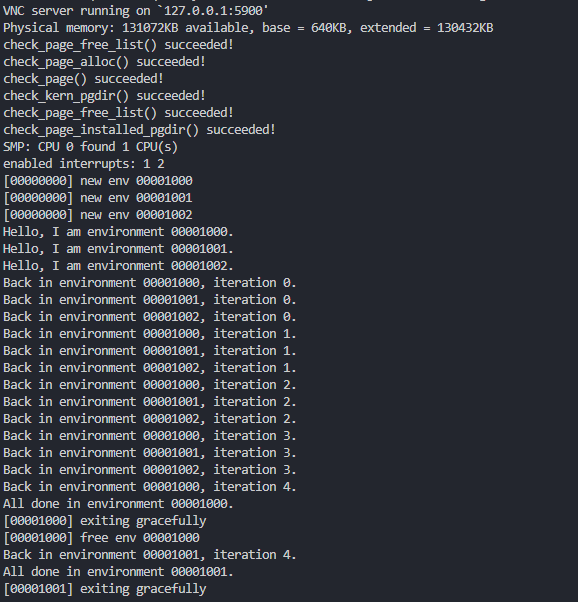
\includegraphics[width=0.5\textwidth]{ex6-1} \par
}
\newpage
若以 \textsl{make qemu CPUS=2} 命令启用双核系统,得到的运行结果如下:\par 
\quad \par  
{
\centering
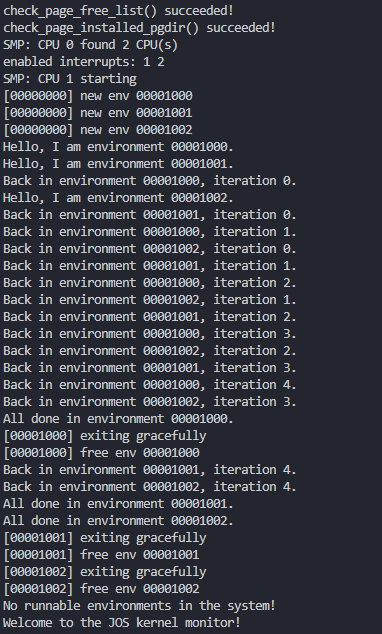
\includegraphics[width=0.5\textwidth]{ex6-2} \par
}
\quad \par 
\question{3}{
    {
        \par 
        3. In your implementation of env\_run() you should have called lcr3(). 
        Before and after the call to lcr3(), your code makes references 
        (at least it should) to the variable e, 
        the argument to env\_run. Upon loading the \%cr3 register, 
        the addressing context used by the MMU is instantly changed. 
        But a virtual address (namely e) has meaning relative to a given address 
        context--the address context specifies the physical address to which 
        the virtual address maps. 
        Why can the pointer e be dereferenced both before and after the addressing switch?
    }
    {
        \par 
        4. Whenever the kernel switches from one environment to another, 
        it must ensure the old environment's registers 
        are saved so they can be restored properly later. 
        Why? Where does this happen?
    }
}

第一个问题的答案很简单:所有的进程都映射了完整的VAS的内核部分,而envs的映射也位于内核
部分中,故所有进程对于envs数组任一进程的地址翻译都是相同的。\par 
第二个问题:进程的现场保存发生在 \_alltrap 过程中,现场恢复发生在 env\_pop\_tf() 时。

\newpage
\section[\large System Calls for Environment Creation]{System Calls for Environment Creation}
目前我们的系统已经可以完成用户态进程的调度了,但我们还未提供真正的用户态使用进程的接口。这一节
我们将实现其中最基础的一部分。提供给用户的进程接口同样采用系统调用的实现方式。\par 

\exercise{7}{
    \par 
    {
        Implement the system calls described above in kern/syscall.c and 
        make sure syscall() calls them. 
        You will need to use various functions in kern/pmap.c and kern/env.c, 
        particularly envid2env(). 
        For now, whenever you call envid2env(), 
        pass 1 in the checkperm parameter. 
        Be sure you check for any invalid system call arguments, 
        returning -E\_INVAL in that case. 
        Test your JOS kernel with user/dumbfork and make sure it works 
        before proceeding.
    } \par
}

\subsection{\large sys\_exofork}
sys\_exofork()函数可以用于创建新的子进程,并且设置子进程的内存映射、
寄存器状态与父进程完全一致(按照状态机复制理解)。对于父子进程而言,函数返回不同的
值(父进程得到子进程的env\_id,子进程返回0):\par
(注:返回值的设置应回忆syscall的调用流与env状态保存逻辑;对于子进程而言,当它
被调度时看起来“就像刚从系统调用返回”一样) 

\lstset{style=CStyle}
\setmainfont{Consolas}
\begin{lstlisting}
static envid_t
sys_exofork(void)
{
    // Create the new environment with env_alloc(), from kern/env.c.
    // It should be left as env_alloc created it, except that
    // status is set to ENV_NOT_RUNNABLE, and the register set is copied
    // from the current environment -- but tweaked so sys_exofork
    // will appear to return 0.

    // LAB 4: Your code here.
    struct Env *new_env;
    int r = env_alloc(&new_env, curenv->env_id);
    if(r  < 0)
        return r;
    
    new_env->env_status = ENV_NOT_RUNNABLE;
    new_env->env_tf = curenv->env_tf;
    new_env->env_tf.tf_regs.reg_eax = 0;

    return new_env->env_id;
}
\end{lstlisting}
\setmainfont{Times New Roman}

\newpage
\subsection{\large sys\_page\_alloc}
sys\_page\_alloc()系统调用为用户提供申请物理页的接口,并映射到指定的
虚拟地址位置。
\lstset{style=CStyle}
\setmainfont{Consolas}
\begin{lstlisting}
static int
sys_page_alloc(envid_t envid, void *va, int perm)
{
    ...
    // LAB 4: Your code here.
    struct Env *e;
    int r = envid2env(envid, &e, 1);

    // bad-env
    if(r < 0)
        return r;
    
    // va is not page-aligned or va >= UTOP
    if((uintptr_t)va >= UTOP || (uintptr_t)va != ROUNDDOWN((uintptr_t)va, PGSIZE))
        return -E_INVAL;

    // perm inappropriate
    if( 
        !(perm & PTE_U) ||
        !(perm & PTE_P) ||
        ((perm | PTE_SYSCALL) != PTE_SYSCALL)
        )
        return -E_INVAL;

    struct PageInfo *pp = page_alloc(0);
    if(!pp)
        return -E_NO_MEM;
    r = page_insert(e->env_pgdir, pp, va, perm);
    if(r < 0)
    {
        page_free(pp);
        return r;
    }

    return 0;

}
\end{lstlisting}
\setmainfont{Times New Roman}

\newpage
\subsection{\large sys\_page\_map}
sys\_page\_map() 系统调用用于将源进程srcva处映射的物理页映射到目的进程
dstva处。需要注意的是若源进程中该物理页为read-only权限,在目的进程中也应保持其只读性。\par 
\lstset{style=CStyle}
\setmainfont{Consolas}
\begin{lstlisting}
static int
sys_page_map(envid_t srcenvid, void *srcva,
            envid_t dstenvid, void *dstva, int perm)
{
    // LAB 4: Your code here.
    struct Env *srcE, *dstE;
    // bad-env
    if(envid2env(srcenvid, &srcE, 1) < 0 ||
       envid2env(dstenvid, &dstE, 1) < 0)
    { return -E_BAD_ENV; }
    // va-error
    if((uintptr_t)srcva >= UTOP || 
       (uintptr_t)srcva != ROUNDDOWN((uintptr_t)srcva, PGSIZE) ||
       (uintptr_t)dstva >= UTOP || (uintptr_t)dstva != ROUNDDOWN((uintptr_t)dstva, PGSIZE))
    { return -E_INVAL; }
    // perm inappropriate
    if( 
        !(perm & PTE_U) || !(perm & PTE_P) ||
        ((perm | PTE_SYSCALL) != PTE_SYSCALL)
    )
    { return -E_INVAL; }

    pte_t *srcPTE;
    struct PageInfo *srcpp = page_lookup(srcE->env_pgdir, srcva, &srcPTE);
    struct PageInfo *dstpp = page_alloc(0);

    // write on read-only
    if((perm & PTE_W) && !(*srcPTE & PTE_W))
        return -E_INVAL;

    // srcva not mapped
    if(!srcpp)
        return -E_INVAL;

    // no memory
    if(page_insert(dstE->env_pgdir, srcpp, dstva, perm) < 0)
        return -E_NO_MEM;
    return 0;
}
\end{lstlisting}
\setmainfont{Times New Roman}

\newpage
\subsection{\large sys\_page\_unmap}
sys\_page\_unmap()系统调用是解除va处的物理页映射,相当于对内核中
page\_remove() 接口的用户态封装。\par 

\lstset{style=CStyle}
\setmainfont{Consolas}
\begin{lstlisting}
static int
sys_page_unmap(envid_t envid, void *va)
{
    // Hint: This function is a wrapper around page_remove().

    // LAB 4: Your code here.
    struct Env *e;
    if(envid2env(envid, &e, 1) < 0)
        return -E_BAD_ENV;
    if((uintptr_t)va >= UTOP || (uintptr_t)va != ROUNDDOWN((uintptr_t)va, PGSIZE))
        return -E_INVAL;
    
    page_remove(e->env_pgdir, va);
    return 0;

}
\end{lstlisting}
\setmainfont{Times New Roman}

\subsection{\large sys\_env\_set\_status}
sys\_env\_set\_status() 用于设置目标进程的运行状态(可运行/不可运行):\par 
\lstset{style=CStyle}
\setmainfont{Consolas}
\begin{lstlisting}
static int
sys_env_set_status(envid_t envid, int status)
{
    // LAB 4: Your code here.
    if(status != ENV_RUNNABLE && status != ENV_NOT_RUNNABLE)
        return -E_INVAL;
    struct Env *e;
    int r = envid2env(envid, &e, 1);
    if(r < 0)
        // error happened
        return r;
    e->env_status = status;
    // when go back to trap() who called this function,
    // the sched_yield will be called
    return 0;

}
\end{lstlisting}
\setmainfont{Times New Roman}

\newpage
完成上述函数实现后,修改syscall()函数的dispatch部分:\par 
\lstset{style=CStyle}
\setmainfont{Consolas}
\begin{lstlisting}
int32_t
syscall(uint32_t syscallno, uint32_t a1, uint32_t a2, uint32_t a3, uint32_t a4, uint32_t a5)
{
    // Call the function corresponding to the 'syscallno' parameter.
    // Return any appropriate return value.
    // LAB 3: Your code here.

    // panic("syscall not implemented");

    switch (syscallno) 
    {
        case SYS_cputs:
            sys_cputs((char *)a1, a2);
            return 0;
        case SYS_cgetc:
            return sys_cgetc();
        case SYS_getenvid:
            return sys_getenvid();
        case SYS_env_destroy:
            return sys_env_destroy(a1);
        case SYS_yield:
            sys_yield();
            return 0;
        case SYS_exofork:
            return sys_exofork();
        case SYS_env_set_status:
            return sys_env_set_status(a1, a2);
        case SYS_page_alloc:
            return sys_page_alloc(a1, (void *)a2, a3);
        case SYS_page_map:
            return sys_page_map(a1, (void *)a2, a3, (void *)a4, a5);
        case SYS_page_unmap:
            return sys_page_unmap(a1, (void *)a2);
        default:
            return -E_INVAL;
    }
}
\end{lstlisting}
\setmainfont{Times New Roman}

% ---- part B ----

\chapter[\Large Copy-on-Write Fork]{Copy-on-Write Fork}
本节实现 fork() 等用户态进程创建的相关调用。JOS在实现fork()调用的时候采用了与xv6不同的方法:
对创建的子进程的地址空间复制采用copy-on-write的方法,即创建时子进程直接复制使用父进程的地址映射
(而不复制内存空间内容本身),等到父子进程任一一方执行写操作引发page fault,再进行内存空间的复制。
这样做的好处是在很多workload中,fork得到的子进程很快就会进行excute操作,而前面耗时复制的父进程地址空间
内容并不起到什么作用;采用copy-on-write可以有效解决这里的性能问题。\par

\section[\large User-level page fault handling]{User-level page fault handling}

JOS 将 page fault 的处理逻辑交给用户态程序定义。用户态进程定义的handler可以使用JOS系统调用的方法来处理
可能出现在该进程上的page fault。

\subsection{Setting the Page Fault Handler}
\exercise{8}{
    \par 
    {
        Implement the sys\_env\_set\_pgfault\_upcall system call. 
        Be sure to enable permission checking when looking up the environment ID of the target 
        environment, since this is a "dangerous" system call.
    } \par
}
这个练习要求我们实现设置 pgfault\_upcall 的函数。pgfault\_upcall 是对 page fault handler 的封装
(详见后文Exercise 10),在执行真正的handler前完成必要的准备工作与善后工作。JOS为env结构体添加了存放
upcall函数的指针,我们只需将用户态传递来的指针设置即可。\par
(注:完成该系统调用同样需要修改syscall的dispatch部分,此处省略)
\newpage
\lstset{style=CStyle}
\setmainfont{Consolas}
\begin{lstlisting}
static int
sys_env_set_pgfault_upcall(envid_t envid, void *func)
{
    // LAB 4: Your code here.
    struct Env *e;
    if(envid2env(envid, &e, 1) < 0)
        return -E_BAD_ENV;
    e->env_pgfault_upcall = func;

    return 0;
}
\end{lstlisting}
\setmainfont{Times New Roman}

\subsection{Normal and Exception Stacks in User Environments}
在调用page fault handler时,JOS还涉及一次栈的切换。当用户态程序正常运行时,它会使用
用户栈(即[USTACKTOP-PGSIZE, STACKTOP)区域)。当 page fault发生时,JOS将栈切换到地址空间
中的用户异常栈([UXSTACKTOP-PGSIZE, UXSTACKTOP))。Hanlder在这个栈上处理page fault,通过
JOS的系统调用执行为缺页提供新的物理页等方式解决page fault。最后Handler退出,用户态程序回到
原有的用户栈处。
\subsection{Invoking the User Page Fault Handler}
与陷入trap时我们在内核栈上维护了Trapframe结构同理,当page fault发生时我们也在上述用户异常栈
上维护一个UTrapframe结构保存发生page fault时的用户态程序现场。当handler结束调用后,我们可以利用
保存的现场恢复原有用户态进程的运行。这一过程是由接管所有page fault trap处理的page\_fault\_handler()
函数完成的:我们在Lab3中实现了对内核态page fault的处理(crash),本节我们需要按照上述想法实现用户态的处理。\par

\subsection{Setting the Page Fault Handler}
\exercise{9}{
    \par 
    {
        Implement the code in page\_fault\_handler in kern/trap.c 
        required to dispatch page faults to the user-mode handler. 
        Be sure to take appropriate precautions 
        when writing into the exception stack. 
        (What happens if the user environment runs out of space on the exception stack?)
    } \par
}
根据实验要求,我们完成代码如下:

\newpage
\lstset{style=CStyle}
\setmainfont{Consolas}
\begin{lstlisting}
void
page_fault_handler(struct Trapframe *tf)
{
    ...
    // LAB 4: Your code here.
    if(curenv->env_pgfault_upcall)
	{
		struct UTrapframe *utf;
		// stacked page fault
		if(UXSTACKTOP - PGSIZE <= tf->tf_esp && tf->tf_esp < UXSTACKTOP)
			// remain a sratch space at the top
			utf = (struct UTrapframe*)(tf->tf_esp - sizeof(struct UTrapframe) - 4);
		// first page fault
		else
			utf = (struct UTrapframe*)(UXSTACKTOP - sizeof(struct UTrapframe));

		// (1) didn't allocate a page for exception stack
		// (2) exception stack overflows
		// (3) can't write it
		user_mem_assert(curenv, (void *)utf, sizeof(struct UTrapframe), PTE_W);

		utf->utf_esp = tf->tf_esp;
		utf->utf_eflags = tf->tf_eflags;
		utf->utf_eip = tf->tf_eip;
		utf->utf_regs = tf->tf_regs;
		utf->utf_err = tf->tf_err;
		utf->utf_fault_va = fault_va;
		
		tf->tf_esp = (uintptr_t)utf;
		tf->tf_eip = (uintptr_t)(curenv->env_pgfault_upcall);
		env_run(curenv);
	}

    // Destroy the environment that caused the fault.
    cprintf("[%08x] user fault va %08x ip %08x\n",
        curenv->env_id, fault_va, tf->tf_eip);
    print_trapframe(tf);
    env_destroy(curenv);
}
\end{lstlisting}
\setmainfont{Times New Roman}

关于这部分代码,有几点需要说明:\par 
首先是判断upcall函数是否存在(用户态程序是否正确设置handler),
如不存在说明用户态程序没有准备处理page fault的程序,
因此我们直接回收进程(根据实验提示,我们在进程回收前打印信息方便调试)。\par 
第二,若upcall函数存在,则第一个要考虑的问题是构造UTrapframe的位置。
我们检查Trapframe为我们提供的发生page fault时ESP的值:如果它已经位于用户异常栈
中,则我们在当前栈中继续生长(根据实验提示,在栈上添加一个字长的空白区域);否则,
我们需要切换到用户异常栈栈顶处。需要注意的是,page\_fault\_handler并不负责用户异常栈
内存的分配(从后续实验可知,这一步交给了用户自定义的handler完成)。\par 
在确定UTrapframe放置位置后,我们填充该结构,并将Trapframe的EIP切换到upcall函数上再调度,
返回用户态后,用户进程开始执行upcall函数。

\subsection{User-mode Page Fault Entrypoint}
\exercise{10}{
    \par 
    {
        Implement the \_pgfault\_upcall routine in lib/pfentry.S. 
        The interesting part is returning to the original point in the user code 
        that caused the page fault. 
        You'll return directly there, 
        without going back through the kernel. 
        The hard part is simultaneously switching stacks and re-loading the EIP.
    } \par
}
在上一个Exercise中,我们在内核态中设置了用户异常栈、将执行流位置设置到upcall函数后
返回到发生了page fault的用户态进程。因此,\underline{整个upcall函数都是运行在用户态下的}。
如前文所述,upcall函数是对用户自定义page fault handler的一个封装:它的主要任务是在调用handler
以后恢复进程现场,使进程重新恢复到触发page fault时的状态。根据实验提示,我们对它的实现如下:\par 
\lstset{style=AssemblyStyle}
\setmainfont{Consolas}
\begin{lstlisting}
.text
.globl _pgfault_upcall
_pgfault_upcall:
    // Call the C page fault handler.
    pushl %esp			// function argument: pointer to UTF
    movl _pgfault_handler, %eax
    call *%eax
    addl $4, %esp			// pop function argument

    // LAB 4: Your code here.
    movl 0x28(%esp), %eax	// take out the trap-time eip
    subl $4, 0x30(%esp)     // page fault address
    movl 0x30(%esp), %edx	// take out the trap-time esp
    movl %eax, (%edx)       // push EIP into USER-STACK
    addl $8, %esp
    popal
    addl $4, %esp
    popfl
    popl %esp
    ret
\end{lstlisting}
\setmainfont{Times New Roman}
\par 
我们同样来理解一下\_pgfault\_upcall的实现。第一部分非我们实现的内容是对
用户定义的handler的调用。我们在这个Exercise中实现的内容是现场的恢复。根据实验的提示,
直接使用jmp指令进行跳转是不可行的:我们需要恢复所有的寄存器现场,如果使用jmp的话我们总是
会需要再一个额外的、不需要恢复的寄存器来保存跳转地址,这会导致恢复的现场与实际现场不一致。
根据实验的提示,我们采用ret指令来回到原来的状态。在Lab3时我们已经接触过,ret指令会将在栈上
的EIP弹出并载入,从而使我们能够回到原初的状态。\par 
我们的代码首先将用户栈和发生page fault时的EIP取出(均存在UTrapframe中),并将EIP放入用户栈中
(注意需先将EIP地址减去4,才是发生page fault的正确地址);之后我们跳过栈顶两个与寄存器现场恢复
无关的值后,popal/popfl恢复现场。最后我们用popl将存放在异常栈栈顶的用户栈地址弹出,进程即成功
切换到用户栈。此时用户栈栈顶存放着page fault发生地址,我们只需ret即可回到现场。\par
\quad \par 
\exercise{11}{
    \par 
    {
        Finish set\_pgfault\_handler() in lib/pgfault.c.
    } \par
}
最后我们要实现注册handler的用户library函数。该函数本身是用户态函数,
因此所有与JOS的交互通过系统调用来执行。在函数第一次被调用时,我们使用
系统调用为用户异常栈分配一个物理页并完成映射,同时将upcall函数设置为
我们在上一个Exercise中实现的\_pgfault\_upcall。upcall函数会根据函数指针名
找到\_pgfault\_handler并执行。\par 
\lstset{style=CStyle}
\setmainfont{Consolas}
\begin{lstlisting}
void
set_pgfault_handler(void (*handler)(struct UTrapframe *utf))
{
    int r;

    if (_pgfault_handler == 0) 
    {
        // First time through!
        // LAB 4: Your code here.
        envid_t envid = sys_getenvid();
        if(sys_page_alloc(envid, (void *)(UXSTACKTOP-PGSIZE), PTE_W | PTE_U | PTE_P) < 0)
            panic("sys_page_alloc failed.");
        if(sys_env_set_pgfault_upcall(envid, _pgfault_upcall) < 0)
            panic("sys_env_set_pgfault_upcall failed.");
    }

    // Save handler pointer for assembly to call.
    _pgfault_handler = handler;
}
\end{lstlisting}
\setmainfont{Times New Roman}

\newpage
\section[\large Implementing Copy-on-Write Fork]{Implementing Copy-on-Write Fork}
\exercise{12}{
    \par 
    {
        Implement fork, duppage and pgfault in lib/fork.c.
        Test your code with the forktree program. 
        It should produce the following messages, with interspersed 'new env', 
        'free env', and 'exiting gracefully' messages. 
        The messages may not appear in this order, and the environment IDs may be different.
    } \par
}
这一节中我们需要实现duppage,pgfault以及完整的fork函数,完成这一个Exercise后我们就可以在用户态创建新进程了。
我们按照duppage,fork到pgfault的顺序实现上述函数。\par 

\subsection{duppage}
duppage()函数用于在指定的进程上完成对某个物理页的映射复制。其使用场景是父进程fork时调用该函数,
将目标页映射复制到子进程VAS中,同时若该页原本为可写页,将父子进程的该映射都设置为copy-on-write模式。

\lstset{style=CStyle}
\setmainfont{Consolas}
\begin{lstlisting}
static int
duppage(envid_t envid, unsigned pn)
{
    // LAB 4: Your code here.
    // map for child
    if((uvpt[pn] & PTE_W) || (uvpt[pn] & PTE_COW))
    {
        int r = sys_page_map(0, (void *)(pn*PGSIZE),envid, (void *)(pn*PGSIZE), 
                             PTE_COW | PTE_U | PTE_P);
        if(r < 0)
            return -1;
        
        // remap for thisenv
        r = sys_page_map(0, (void *)(pn*PGSIZE), 0, (void *)(pn*PGSIZE),
                         PTE_COW | PTE_U | PTE_P);
        if(r < 0)
            return -1;
    }
    else
    {
        int r = sys_page_map(0, (void *)(pn*PGSIZE), envid, (void *)(pn*PGSIZE),
                             PTE_U | PTE_P);
        if(r < 0)
            return -1;
    }
    return 0;
}
\end{lstlisting}
\setmainfont{Times New Roman}

\newpage
函数实现上有一个要注意的点:检查需要被dup的页的用户态权限时,用到了在env\_alloc阶段映射在
VAS中的[UVPT, UVPT+PTSIZE)段:这个段映射了用户进程的页目录(见env\_setup\_vm()的实现)。
JOS在entry.S中提供了两个变量:uvpt和uvpd。\par 

\lstset{style=AssemblyStyle}
\setmainfont{Consolas}
\begin{lstlisting}
.globl uvpt
.set uvpt, UVPT
.globl uvpd
.set uvpd, (UVPT+(UVPT>>12)*4)
\end{lstlisting}
\setmainfont{Times New Roman}
\par 这里JOS使用了一个相当trick的方法:将页目录作为页表进行查询,
从而得到页目录/页表自身。将UVPT段映射到页目录自身的物理地址后,x86对PDX与UVPT相同的段进行地址翻译时,根据对应的PDE找到自身,在第二步翻译时
实际上是根据PTX对页目录进行搜索,根据PTX偏移量得到的正是对应页表的PTE。JOS定义了一个虚拟地址为UVPT的数组uvpt,作为页表访问入口。\par 
如果需要访问页目录呢?在访问页表时首先需要确定页表是否存在,这是记录在PDE中的。实际访问逻辑与上述访问页表逻辑是相同的,只需将地址的PDX与PTX都
设置为与UVPT的PDX段相同即可。JOS定义了数组uvpd,虚拟地址为(UVPT+(UVPT >> PGSHIFT)*4)。\par
(注:页目录/页表与页的寻址方式不同:页目录与页表按照字(JOS中即4字节寻址),而物理页按照字节寻址。在定义uvpt和uvpd变量
时将它们定义为了pte\_t和pde\_t数组,因此索引时得到实际地址应为uvpt/uvpd基址加上4*下标偏移量。对于uvpt,下标偏移量计算使用
PGNUM(addr),而对于uvpd则为PDX(addr)。)\par 

\quad \par  
{
\centering
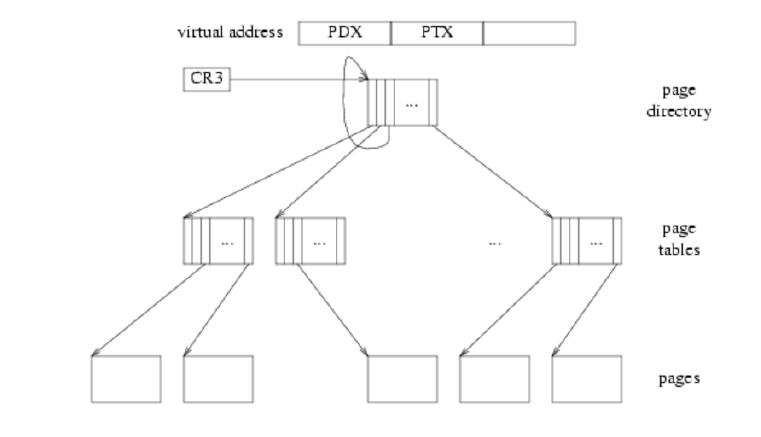
\includegraphics[width=0.9\textwidth]{uvpt} \par
}

\newpage

\subsection{fork}
\lstset{style=CStyle}
\setmainfont{Consolas}
\begin{lstlisting}
envid_t
fork(void)
{
    // LAB 4: Your code here.
    set_pgfault_handler(pgfault);
    envid_t newChildId = sys_exofork();
    if(newChildId < 0)
        return -1;
    
    // for child-process
    if(newChildId == 0)
    {
        thisenv = envs + ENVX(sys_getenvid());
        return 0;
    }

    // allocate a page for child-exception-stack
    if(sys_page_alloc(newChildId, (void *)(UXSTACKTOP-PGSIZE), PTE_W | PTE_U | PTE_P) < 0)
        return -1;
    
    // set child-pgfault-upcall
    sys_env_set_pgfault_upcall(newChildId, (void *)_pgfault_upcall);

    // copy the map into child
    uintptr_t addr;
    for(addr = 0; addr < USTACKTOP; addr += PGSIZE)
        if((uvpd[PDX(addr)] & PTE_P) && (uvpt[PGNUM(addr)] & PTE_P))
            duppage(newChildId, PGNUM(addr));

    // set child to be runnable
    if(sys_env_set_status(newChildId, ENV_RUNNABLE) < 0)
        return -1;

    return newChildId;
}
\end{lstlisting}
\setmainfont{Times New Roman}

fork实现时依次完成几件事:
(1) 创建子进程(此时子进程仍未NOT\_RUNNABLE);
(2) 从子进程返回时修改thisenv后直接返回(这一步会在父进程昨晚所有处理、将子进程设置为RUNNABLE后才可能被调度执行);
(3) 为子进程分配独立的用户异常栈(不使用cow);
(4) 对所有VAS中的用户态内存进行cow-dup;
(5) 将子进程设置为可被调度运行的状态后返回。
\par 

\newpage
\subsection{pgfault}

\lstset{style=CStyle}
\setmainfont{Consolas}
\begin{lstlisting}
static void
pgfault(struct UTrapframe *utf)
{
    void *addr = (void *) utf->utf_fault_va;
    uint32_t err = utf->utf_err;
    int r;

    // Check that the faulting access was (1) a write, and (2) to a
    // copy-on-write page.  If not, panic.
    // Hint:
    //   Use the read-only page table mappings at uvpt
    //   (see <inc/memlayout.h>).

    // LAB 4: Your code here.
    if(!((uvpt[PGNUM(addr)] & PTE_COW) && (err & FEC_WR))
    )
    { panic("pgfault panic!"); }

    // Allocate a new page, map it at a temporary location (PFTEMP),
    // copy the data from the old page to the new page, then move the new
    // page to the old page's address.
    // Hint:
    //   You should make three system calls.

    // LAB 4: Your code here.
    envid_t envId = sys_getenvid(); // Don't use curenv->env_id!
    if(sys_page_alloc(envId, (void *)(PFTEMP), PTE_P | PTE_U | PTE_W) < 0)
        panic("sys_page_alloc failed in pgfault().");

    // memory-move
    memmove((void *)PFTEMP, (void *)(ROUNDDOWN(addr, PGSIZE)), PGSIZE);

    if(sys_page_map(
        envId, (void *)(PFTEMP), 
        envId, (void *)(ROUNDDOWN(addr, PGSIZE)),
        PTE_P | PTE_W | PTE_U) < 0
    )
    { panic("sys_page_map failed in pgfault().");; }

    if(sys_page_unmap(envId, (void *)(PFTEMP)) < 0)
        panic("sys_page_unmap failed in pgfault().");
}
\end{lstlisting}
\setmainfont{Times New Roman}

\newpage
该函数即为默认的page fault处理函数。当发生的错误是对cow页进行写操作时,
创建新的物理页,对原始页进行复制操作。这里借用了VAS中的临时区域PFTEMP作为临时
位置,协助进行物理页内容的移动。

\chapter[\Large Preemptive Multitasking and Inter-Process communication (IPC)]{Preemptive Multitasking and Inter-Process communication (IPC)}

\section[\large Clock Interrupts and Preemption]{Clock Interrupts and Preemption}
本节要求我们利用时钟中断实现抢断式的任务调度。在目前JOS的完成进度上,
OS并没有任何主动手段可以从正在运行中的用户进程手中重新获取执行权,只能等待
用户进程执行完后回收或调用 sys\_yield() 主动让渡出CPU。我们在这节实验中要
实现抢占式调度,也即在每次时钟中断发生时,OS重新获得执行权并进行新一轮的进程调度
(根据PartA内容,JOS执行Round-robin调度)。\par 
在JOS中,处于内核态时会关闭外部中断,仅在用户进程执行时开启中断。外部中断由IRQs表示,
其中IRQ 0为时钟中断。\par 

\subsection{Interrupt discipline}

\exercise{13}
{
    \par
    {
        Modify kern/trapentry.S and kern/trap.c to initialize 
        the appropriate entries in the IDT and 
        provide handlers for IRQs 0 through 15. 
        Then modify the code in env\_alloc() in kern/env.c 
        to ensure that user environments are always run 
        with interrupts enabled.
    }
    \par
    {
        Also uncomment the sti instruction in sched\_halt() so that idle CPUs unmask interrupts.
    }
    \par
    
    {
        The processor never pushes an error code when invoking 
        a hardware interrupt handler. 
        You might want to re-read section 9.2 of the 80386 
        Reference Manual, 
        or section 5.8 of the IA-32 Intel Architecture Software 
        Developer's Manual, Volume 3, at this time.
    }
    \par 
    {
        After doing this exercise, 
        if you run your kernel with any test program that runs 
        for a non-trivial length of time (e.g., spin), 
        you should see the kernel print trap frames for 
        hardware interrupts. 
        While interrupts are now enabled in the processor, 
        JOS isn't yet handling them, 
        so you should see it misattribute each interrupt 
        to the currently running user environment and destroy it. 
        Eventually it should run out of environments to destroy 
        and drop into the monitor.
    }
    \par 
}

这节要为IRQs设置trap入口,与我们在Lab3中设置其他
trap入口的方式是一样的。根据提示,IRQs均为无ErrorCode的模式,我们
修改trapentry.S,增加对应的接口函数:\par 

\lstset{style=AssemblyStyle}
\setmainfont{Consolas}
\begin{lstlisting}
/* Add in Lab4 */
TRAPHANDLER_NOEC(IRQ_TIMER_HANDLER,    IRQ_OFFSET + IRQ_TIMER)
TRAPHANDLER_NOEC(IRQ_KBD_HANDLER,      IRQ_OFFSET + IRQ_KBD)
TRAPHANDLER_NOEC(IRQ_SERIAL_HANDLER,   IRQ_OFFSET + IRQ_SERIAL)
TRAPHANDLER_NOEC(IRQ_SPURIOUS_HANDLER, IRQ_OFFSET + IRQ_SPURIOUS)
TRAPHANDLER_NOEC(IRQ_IDE_HANDLER,      IRQ_OFFSET + IRQ_IDE)
TRAPHANDLER_NOEC(IRQ_ERROR_HANDLER,    IRQ_OFFSET + IRQ_ERROR)
\end{lstlisting}
\setmainfont{Times New Roman}
\par
修改trap中设置IDT的部分的代码:\par 
\lstset{style=CStyle}
\setmainfont{Consolas}
\begin{lstlisting}
void
trap_init(void)
{
    extern struct Segdesc gdt[];
    ...
    // Add in Lab4
    extern void IRQ_TIMER_HANDLER();
    extern void IRQ_KBD_HANDLER();
    extern void IRQ_SERIAL_HANDLER();
    extern void IRQ_SPURIOUS_HANDLER();
    extern void IRQ_IDE_HANDLER();
    extern void IRQ_ERROR_HANDLER();
    ...
    // Add in Lab4
    SETGATE(idt[IRQ_OFFSET + IRQ_TIMER], 0, GD_KT, IRQ_TIMER_HANDLER, 0);
    SETGATE(idt[IRQ_OFFSET + IRQ_KBD], 0, GD_KT, IRQ_KBD_HANDLER, 0);
    SETGATE(idt[IRQ_OFFSET + IRQ_SERIAL], 0, GD_KT, IRQ_SERIAL_HANDLER, 0);
    SETGATE(idt[IRQ_OFFSET + IRQ_SPURIOUS], 0, GD_KT, IRQ_SPURIOUS_HANDLER, 0);
    SETGATE(idt[IRQ_OFFSET + IRQ_IDE], 0, GD_KT, IRQ_IDE_HANDLER, 0);
    SETGATE(idt[IRQ_OFFSET + IRQ_ERROR], 0, GD_KT, IRQ_ERROR_HANDLER, 0);
    
    ...
}
\end{lstlisting}
\setmainfont{Times New Roman}

最后再根据提示修改sched\_halt()函数,增加打开中断的指令即可。

\newpage
\subsection{Handling Clock Interrupts}
完成入口设置后,我们再实现时钟中断的handler,实现也比较简单:每次触发IRQ Timer时
使JOS进行一次系统调度即可。\par 
\exercise{14}
{
    \par 
    {
        Modify the kernel's trap\_dispatch() function 
        so that it calls sched\_yield() to find and 
        run a different environment whenever a clock interrupt takes place.
    }
    \par 
    {
        You should now be able to get the user/spin test to work: 
        the parent environment should fork off the child, 
        sys\_yield() to it a couple times but in each case 
        regain control of the CPU after one time slice, 
        and finally kill the child environment and 
        terminate gracefully.
    }
    \par 
}

\lstset{style=CStyle}
\setmainfont{Consolas}
\begin{lstlisting}
static void
trap_dispatch(struct Trapframe *tf)
{
    ...
    // Handle clock interrupts. Don't forget to acknowledge the
    // interrupt using lapic_eoi() before calling the scheduler!
    // LAB 4: Your code here.
    if (tf->tf_trapno == IRQ_OFFSET + IRQ_TIMER) {
        lapic_eoi();
        sched_yield();
    }

    ...
}
\end{lstlisting}
\setmainfont{Times New Roman}

\section[\large Inter-Process communication (IPC)]{Inter-Process communication (IPC)}
这一节要求我们完成JOS的进程间通信功能。JOS为用户进程提供的进程通信方法由两个系统调用来实现:
sys\_ipc\_try\_send与sys\_ipc\_recv。前者用于向某一envid指定的进程发送消息(方式是传递
一个在当前进程中映射的虚拟地址,JOS找到它对应的物理页,并将其映射到指定进程的VAS中),后者
用于将当前进程设置为接收信息的状态并挂起(挂起前指定接收到的物理页应当映射的VA),直到有
任一进程向其通讯后再重新变为可调度状态。\par 
JOS在user-lib中进一步封装了这两个API,得到:ipc\_send() 与 ipc\_recv()。用户可以直接使用
这两个API进行通信(实例:user/sendpage.c)。\par 

\newpage


\exercise{15}
{
    \par 
    {
        Implement \underline{sys\_ipc\_recv} and \underline{sys\_ipc\_try\_send} in kern/syscall.c. 
        Read the comments on both before implementing them, 
        since they have to work together. 
        When you call envid2env in these routines, 
        you should set the checkperm flag to 0, 
        meaning that any environment is allowed to 
        send IPC messages to any other environment, 
        and the kernel does no special permission 
        checking other than verifying that the target envid is valid.
    }
    \par 
    {
        Then implement the ipc\_recv and ipc\_send functions in lib/ipc.c.
    }
    \par
    {
        Use the user/pingpong and user/primes functions to test your IPC mechanism. 
        user/primes will generate for each prime number a new environment 
        until JOS runs out of environments. 
        You might find it interesting to read user/primes.c 
        to see all the forking and IPC going on behind the scenes.
    }
    \par 
}

\subsection{sys\_ipc\_recv}
该函数负责设置接受新页映射的VA。当设置完成后,进程将被挂起(即暂时不被调度),
直到有某一进程向其通信并设置VA映射后,该进程才重新可调度。\par 
\lstset{style=CStyle}
\setmainfont{Consolas}
\begin{lstlisting}
static int
sys_ipc_recv(void *dstva)
{
    // LAB 4: Your code here.	
    if((uintptr_t)dstva < UTOP && (uintptr_t)dstva != ROUNDDOWN((uintptr_t)dstva, PGSIZE))
        return -E_INVAL;
        
    curenv->env_status = ENV_NOT_RUNNABLE;
    curenv->env_ipc_dstva = dstva;
    curenv->env_ipc_recving = true;
    sched_yield();
    // should not come here
    return 0;
}
\end{lstlisting}
\setmainfont{Times New Roman}
这里有一点需要注意:当调用sched\_yield()后,\underline{实际上进程再次被调用时不会返回该执行点处}
(直接自系统调用处返回),因此在后续我们实现recv的恢复时,应当注意对返回状态的设置问题(见下文send
函数的实现)。

\newpage
\subsection{sys\_ipc\_try\_send}
send函数首先找到srcva处映射的物理页,检查其各flag位符合要求后,将该物理页
映射到通信目标进程指定的dstva处,并将目标进程重新设置为可调度的。需要注意的是:
此处有对目标进程trapFrame-eax寄存器设置的语句(EAX存放trap的返回值)。上文我们
提到,当等待通信的进程再次被调度时,它会直接从系统调用返回,而在recv中我们还未能
正确设置其返回值,因此我们需要在这一步完成对目标进程系统调用返回值的设置。\par 

\lstset{style=CStyle}
\setmainfont{Consolas}
\begin{lstlisting}
static int
sys_ipc_try_send(envid_t envid, uint32_t value, void *srcva, unsigned perm)
{
    // LAB 4: Your code here.
    struct Env *dstEnv;
    // Error1: No dst-env
    if(envid2env(envid, &dstEnv, 0) < 0)
        return -E_BAD_ENV;
    // Error2: dst-env is not recving
    if(!dstEnv->env_ipc_recving)
        return -E_IPC_NOT_RECV;
    // Error3: not page-aligned / not mapped / PTE_W for read-only page
    struct PageInfo *pp;
    pte_t *srcPte;
    pp = page_lookup(curenv->env_pgdir, srcva, &srcPte);
    if(
        (uintptr_t)srcva < UTOP &&
        ((uintptr_t)srcva != ROUNDDOWN((uintptr_t)srcva, PGSIZE) ||
        !pp || ((perm & PTE_W) && !(*srcPte & PTE_W)) ||
        !(perm & PTE_U) || !(perm & PTE_P) || (perm & (~PTE_SYSCALL)))
    ){ return -E_INVAL; }

    int r;
    if(
        (uintptr_t)srcva < UTOP && 
        (r = page_insert(dstEnv->env_pgdir, pp, dstEnv->env_ipc_dstva, perm) < 0)
    ){ return r; }

    dstEnv->env_ipc_recving = false;
    dstEnv->env_ipc_from = curenv->env_id;
    dstEnv->env_ipc_value = value;
    dstEnv->env_ipc_perm = perm;
    dstEnv->env_status = ENV_RUNNABLE;
    dstEnv->env_tf.tf_regs.reg_eax = 0;  // !
    return 0;
    
}
\end{lstlisting}
\setmainfont{Times New Roman}

\newpage
\subsection{ipc\_recv}
该lib函数是对系统调用recv的一层封装。需要注意的点是:
当指定的地址pg为0的时候,我们无法完成正确的通信,而且
我们需要将这一点传达给send函数(忽略此次通信)。设置为0
的地址并不能完成这一点。根据我们上面对两个系统调用的实现,
我们可以将pg设置为边界值UTOP,这样系统调用将自然返回。\par 
\lstset{style=CStyle}
\setmainfont{Consolas}
\begin{lstlisting}
int32_t
ipc_recv(envid_t *from_env_store, void *pg, int *perm_store)
{
    // LAB 4: Your code here.
    if(pg == NULL)
        pg = (void *)UTOP;

    int r = sys_ipc_recv(pg);
    if(r < 0)
    {
        if(from_env_store)
            *from_env_store = 0;
        if(perm_store)
            *perm_store = 0;
        return r;
    }
    if(from_env_store)
        *from_env_store = thisenv->env_ipc_from;
    if(perm_store)
        *perm_store = thisenv->env_ipc_perm;
    
    return thisenv->env_ipc_value;
}
\end{lstlisting}
\setmainfont{Times New Roman}

\newpage

\subsection{ipc\_send}
send函数的lib-version实现也是同理。(未解决:为什么使用while)
\lstset{style=CStyle}
\setmainfont{Consolas}
\begin{lstlisting}
void
ipc_send(envid_t to_env, uint32_t val, void *pg, int perm)
{
    // LAB 4: Your code here.
    if(pg == NULL)
        pg = (void *)UTOP;

    int r;
    while((r = sys_ipc_try_send(to_env, val, pg, perm)) < 0)
    {
        if(r != -E_IPC_NOT_RECV)
            panic("ipc_send error: sys_ipc_try_send failed.");
        sys_yield();
    }
}
\end{lstlisting}
\setmainfont{Times New Roman}

\end{document}